\documentclass[addpoints]{exam}
\usepackage{amsmath,amsthm,amssymb,url}

\usepackage{algorithm}
\usepackage{algorithmic}
\usepackage{graphicx}
\usepackage{float}
\usepackage{units}
%\usepackage{algpseudocode}

\usepackage[pdftex]{hyperref}
\usepackage{tikz}
\usepackage{pgfplots}
\usetikzlibrary{calc,3d,decorations.markings, backgrounds, positioning,intersections,shapes}

\renewcommand{\algorithmicrequire}{\textbf{Input:}}
\renewcommand{\algorithmicensure}{\textbf{Output:}}
%\algnewcommand\algorithmicparfor{\textbf{parallel for}}
%\algdef{S}[FOR]{PFOR}[1]{\algorithmicparfor\ #1\ \algorithmicdo}

\newcommand{\BigO}[1]{\mathcal{O}\left( #1\right)}
\newcommand{\ceil}[1]{\left \lceil #1 \right \rceil }
\newcommand{\floor}[1]{\left \lfloor #1 \right \rfloor }


\newtheorem{lemma}{Lemma}[section]
\newcommand{\var}{\text{Var}}
\title{CS 6230: Homework 3}
\date{Due Date: February 24, 2016}
\author{Christopher Mertin}
\begin{document}
\maketitle
%\begin{center}
%\fbox{\fbox{\parbox{5.5in}{\centering
%This assignment has \numquestions\ questions, for a total of \numpoints\
%points.
%Unless otherwise specified, complete and reasoned arguments will be
%expected for all answers. 
%}}}
%\end{center}

\qformat{Question \thequestion: \thequestiontitle\dotfill}
\pointname{}
\bonuspointname{}
\pointformat{[\bfseries\thepoints]}

\printanswers



\begin{questions}

\titledquestion{Computing the Median}
Using the work-depth language, give an algorithm for computing the median of an unsorted array of $n$ integers. What is the work and depth of your algorithm? Is your algorithm work optimal? Suggest how you would find the $k$-ranked element in an unsorted array.

[{\em Hint:} The median is the $k=n/2$-ranked element]

\begin{solution}
The algorithm for this is known as {\em QuickSelect} was taken from \cite{qselect} and made parallel. The algorithm is a Randomized Algorithm and is able to find the $k^{th}$ element in $\BigO{n}$ time. The parallel version of \verb~QuickSelect~ can be seen in Algorithm~\ref{alg:qselect}.

\begin{algorithm}[H]
\centering
\caption{QuickSelect($A$,$k$)}
\begin{algorithmic}[1]
\REQUIRE{$A\in \mathbb{R}^{n\times 1}$ and $k^{th}$-element}
\ENSURE{Index of $k^{th}$-element}
\STATE{$r\leftarrow$ Chosen uniformly at random from $[1,A.size()]$}
\STATE{$pivot \leftarrow A[r]$}
\STATE{$A_{1}, A_{2}$ are new arrays}
\COMMENT{Split into a pile $A_{1}$ small elements and $A_{2}$ large elements}
\STATE{\#pragma omp parallel for}
\FOR{$i=1$ \TO $n$}
    \IF{$A[i] < pivot$}
       \STATE{$A_{1}.append(A[i])$}
    \ELSE
       \IF{$A[i] > pivot$}
          \STATE{$A_{2}.append(A[i])$}
       \ELSE
          \STATE{do nothing}
       \ENDIF
   \ENDIF
\ENDFOR
\IF{$k \leq A_{1}.size()$}
   \RETURN{QuickSelect($A_{1}$, $k$)}
   \COMMENT{It's in the pile of small elements}
\ELSE
   \IF{$k > A.size() - A_{2}.size()$}
       \RETURN{QuickSelect($A_{2}$, $k - A.size() - A_{2}.size()$)}
       \COMMENT{It's in the pile of large elements}
   \ELSE
       \RETURN{$pivot$}
   \ENDIF
\ENDIF
\end{algorithmic}
\label{alg:qselect}
\end{algorithm}

By making the for-loop in lines 4--12 parallel, you reduce the work to separating the data by a factor of $p$, where $p$ is the number of processors. This reduces the work to be $\BigO{n}$ as you need to perform $n$-``binnings'' of the data (either the large or small arrays), and the depth is $\BigO{n/p}$. This is work optimal as parallelizing the for-loop does not require anymore work and just decreases the depth of the algorithm.
\end{solution}


\titledquestion{$d$-dimensional Hypercube Reduction}
Generalize the hypercube reduction algorithm for a $d$-dimensional hypercube for the case in which the number of processors is not a power of two and for any problem size $n\geq p$. Derive an expression for the wall-clock time $T(n,p)$ as a function of the number of processors $p$ and the problem size $n$. Your estimate should include communication costs in terms of latency, bandwidth, and message size.

\begin{solution}
The solution to this problem can be simplified in the following way. You do need $2^{d}$ nodes for a $d$-dimensional hypercube, but when you're looking at the network complexity, it is easy to treat {\em all network topologies} as you would similar to that of a hypercube and go from there. For example, a $3$-dimensional hypercube can be represented as

\begin{figure}[H]
  \centering
  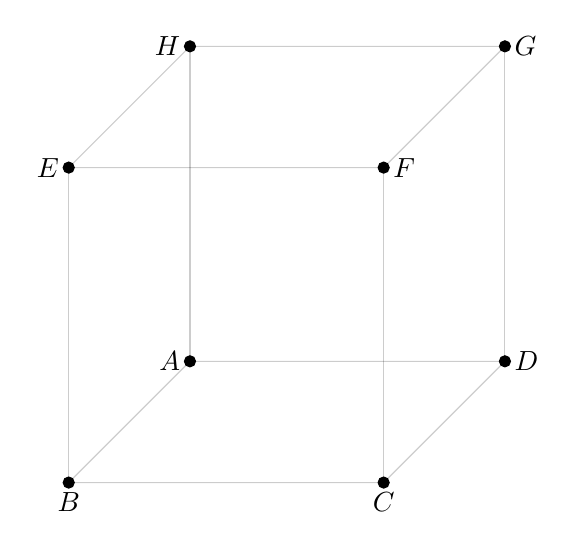
\begin{tikzpicture}[scale=2]
    
    \coordinate (G) at (2,2,0);
    \coordinate (D) at (2,0,0);
    \coordinate (C) at (2,0,2);
    \coordinate (F) at (2,2,2);
    \coordinate (E) at (0,2,2);
    \coordinate (B) at (0,0,2);
    \coordinate (A) at (0,0,0);
    \coordinate (H) at (0,2,0);
    
    \draw[fill=black] (A) circle (1pt) node[anchor=east] {$A$};
    \draw[fill=black] (B) circle (1pt) node[anchor=north] {$B$};
    \draw[fill=black] (C) circle (1pt) node[anchor=north] {$C$};
    \draw[fill=black] (D) circle (1pt) node[anchor=west] {$D$};
    \draw[fill=black] (E) circle (1pt) node[anchor=east] {$E$};
    \draw[fill=black] (F) circle (1pt) node[anchor=west] {$F$};
    \draw[fill=black] (G) circle (1pt) node[anchor=west] {$G$};
    \draw[fill=black] (H) circle (1pt) node[anchor=east] {$H$};
    
    
    \draw[opacity=0.2] (A)--(B)--(C)--(D)--cycle;
    \draw[opacity=0.2] (E)--(F)--(G)--(H)--cycle;
    \draw[opacity=0.2] (A)--(H);
    \draw[opacity=0.2] (B)--(E);
    \draw[opacity=0.2] (D)--(G);
    \draw[opacity=0.2] (C)--(F);

  \end{tikzpicture}
\caption{3-dimensional Hypercube}
\end{figure}

This can be redrawn in a 2-dimensional plane for {\em any} $d$-dimensional hypercube. This doesn't make the compleixty any harder, though does make it easier when designing an algorithm. It can be represented as

\begin{figure}[H]
  \centering
  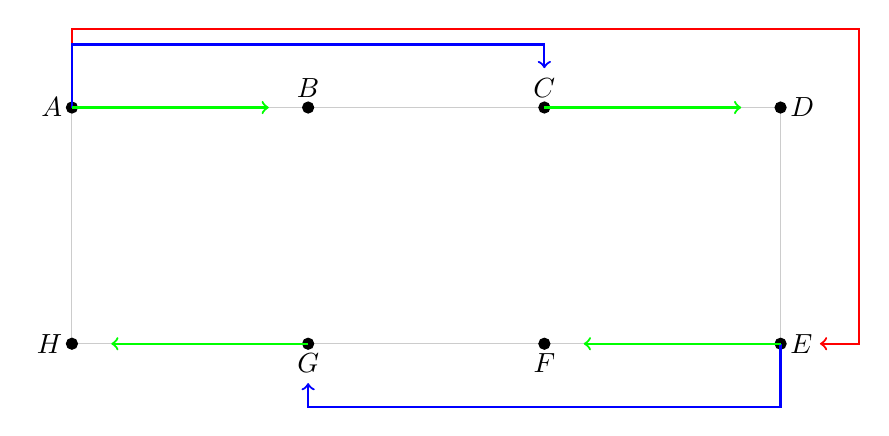
\begin{tikzpicture}[scale=2]
    \coordinate (A) at (0,1.5);
    \coordinate (B) at (1.5,1.5);
    \coordinate (C) at (3,1.5);
    \coordinate (D) at (4.5,1.5);
    \coordinate (E) at (4.5,0);
    \coordinate (F) at (3,0);
    \coordinate (G) at (1.5,0);
    \coordinate (H) at (0,0);

    \draw[fill=black] (A) circle (1pt) node[anchor=east] {$A$};
    \draw[fill=black] (B) circle (1pt) node[anchor=south] {$B$};
    \draw[fill=black] (C) circle (1pt) node[anchor=south] {$C$};
    \draw[fill=black] (D) circle (1pt) node[anchor=west] {$D$};
    \draw[fill=black] (E) circle (1pt) node[anchor=west] {$E$};
    \draw[fill=black] (F) circle (1pt) node[anchor=north] {$F$};
    \draw[fill=black] (G) circle (1pt) node[anchor=north] {$G$};
    \draw[fill=black] (H) circle (1pt) node[anchor=east] {$H$};
    
    \draw[opacity=0.2] (A)--(B)--(C)--(D)--(E)--(F)--(G)--(H)--cycle;
    \draw[->,thick,red] (A)--(0,2)--(5,2)--(5,0)--(4.75,0);
    \draw[blue,->,thick] (E)--(4.5,-.4)--(1.5,-.4)--(1.5,-.25);
    \draw[blue,->,thick] (A)--(0,1.9)--(3,1.9)--(3,1.75);
    \draw[green,->,thick] (A)--(1.25,1.5);
    \draw[green,->,thick] (C)--(4.25,1.5);
    \draw[green,->,thick] (E)--(3.25,0);
    \draw[green,->,thick] (G)--(.25,0);
  \end{tikzpicture}
\caption{3-dimensional Hypercube Communication (One-To-All)}
\end{figure}

which represents the optimal communcation path for a 3-dimensional hypercube. The red represents the data sent during the first clock cycle, the blue is the second clock cycle, and green is the third. While this isn't the {\em reduction}, the reduction algorithm would simply be the reverse of this.

\begin{figure}[H]
  \centering
  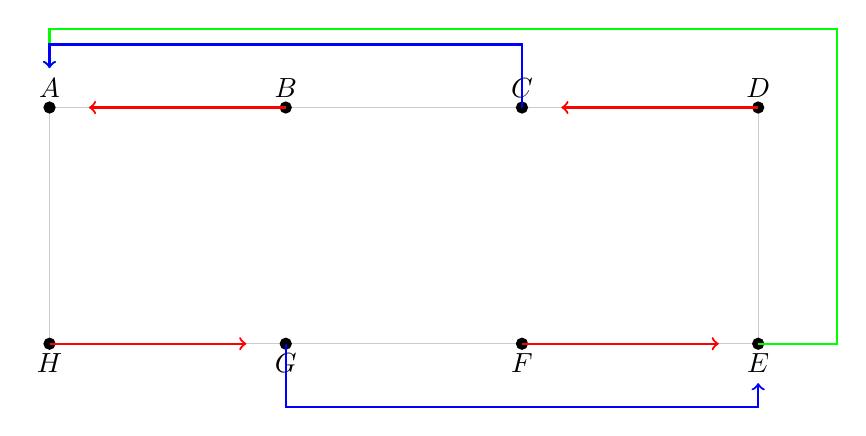
\begin{tikzpicture}[scale=2]
    \coordinate (A) at (0,1.5);
    \coordinate (B) at (1.5,1.5);
    \coordinate (C) at (3,1.5);
    \coordinate (D) at (4.5,1.5);
    \coordinate (E) at (4.5,0);
    \coordinate (F) at (3,0);
    \coordinate (G) at (1.5,0);
    \coordinate (H) at (0,0);

    \draw[fill=black] (A) circle (1pt) node[anchor=south] {$A$};
    \draw[fill=black] (B) circle (1pt) node[anchor=south] {$B$};
    \draw[fill=black] (C) circle (1pt) node[anchor=south] {$C$};
    \draw[fill=black] (D) circle (1pt) node[anchor=south] {$D$};
    \draw[fill=black] (E) circle (1pt) node[anchor=north] {$E$};
    \draw[fill=black] (F) circle (1pt) node[anchor=north] {$F$};
    \draw[fill=black] (G) circle (1pt) node[anchor=north] {$G$};
    \draw[fill=black] (H) circle (1pt) node[anchor=north] {$H$};
    
    \draw[opacity=0.2] (A)--(B)--(C)--(D)--(E)--(F)--(G)--(H)--cycle;
    \draw[->,thick,green] (E)--(5,0)--(5,2)--(0,2)--(0,1.75);
    \draw[blue,->,thick] (G)--(1.5,-.4)--(4.5,-.4)--(4.5,-.25);
    \draw[blue,->,thick] (C)--(3,1.9)--(0,1.9)--(0,1.75);
    \draw[red,->,thick] (B)--(.25,1.5);
    \draw[red,->,thick] (D)--(3.25,1.5);
    \draw[red,->,thick] (F)--(4.25,0);
    \draw[red,->,thick] (H)--(1.25,0);
  \end{tikzpicture}
\caption{3-dimensional Hypercube Reduction (All-To-One)}
\end{figure}


The pseudocode for the $d$-dimensional hypercube communication can be seen in Algorithm~\ref{alg:hyper_cube}. Note: The inner for-loop for the code is called all at once in practice, and it doesn't iterate through the entire list of nodes. However, this was the best way that I could determine to represent it in algorithmic form. For the hypercube reduction, that can be seen in Algorithm~\ref{alg:hyper_red}. For Algorithm~\ref{alg:hyper_red}, we first assume that each node in the network has been given (or already computed) it's share of the values, meaning that each node has $n/p$ values initially. For the {\em very first clock cycle}, each node will perform the reduction on the data that it already has before entering the for-loop.


\begin{algorithm}[H]
\centering
\caption{Hypercube Communication (One-To-All)}
\begin{algorithmic}[1]
\FOR{$i=1$ \TO $\log_{2}(p)$}
    \FOR{$j=1$ \TO $p$}
        \IF{$p_{j}$ contains data}
           \STATE{$m = j+1+\floor{\frac{p}{2^{i}}}$}
           \STATE{$SendData\left(p_{j} \rightarrow p_{m}\right)$}
        \ENDIF
    \ENDFOR
\ENDFOR
\end{algorithmic}
\label{alg:hyper_cube}
\end{algorithm}

\begin{algorithm}[H]
\centering
\caption{Hypercube Reduction (All-To-One)}
\begin{algorithmic}[1]
\FORALL{nodes}
    \STATE{Reduce $n/p$ data on each node}
\ENDFOR
\FOR{$i=\log_{2}(p)$ \TO $1$}
    \FOR{$j=1$ \TO $p$}
        \IF{$p_{j}$ contains data}
           \STATE{$m = j-1-\floor{\frac{p}{2^{i}}}$}
           \STATE{$SendData\left(p_{j} \rightarrow p_{m}\right)$}
        \ENDIF
    \ENDFOR
\ENDFOR
\end{algorithmic}
\label{alg:hyper_red}
\end{algorithm}

Again, the inner for-loop is done all at once for those nodes which are supposed to send the data. From this, we can get the time complexity of this algorithm, which we can make the following approximation. Even with $n\geq p$, as long as it isn't such that $n\gg p$ then we can say that the initial reduction is essentially negligable. This is due to the time to reduce the first $n/p$ values would be much less than the communication time. If not, it would be the case that it would take $n/p$ clock cycles which can be added to our final time complexity. From here, we can build the time complexity as being

\begin{align*}
T(n,p) &= \log_{2}(p)\cdot t(s) + \frac{n\cdot m(s)}{bandwidth}
\intertext{where $t(s)$ is the time (in seconds) of the latency, $bandwidth$ is the bandwith of the network in $bytes/second$, $m(s)$ is the size of the message in $bytes$. The $\log_{2}(p)$ term comes about from having to send $\log_{2}(p)$ messages. The more generalized time complexity for $n\gg p$ can be defined as below where $c(s)$ is $clock\ cycles/second$}
T(n,p) &= \log_{2}(p)\cdot t(s) + \frac{n\cdot m(s)}{bandwidth} + \frac{1}{c(s)}\frac{n}{p}
\end{align*}
\end{solution}


\titledquestion{Finding MPI Bugs}
\href{http://www.cs.utah.edu/~hari/teaching/paralg/bugs.zip}{This archive} contains the files \verb~mpi_bug1.c~, \verb~mpi_bug2.c~, ..., \verb~mpi_bug7.c~. These example codes contain bugs, resulting in hangs or other undesirable behavior. Try to find these bugs and fix them. Add a short comment to the code describing what was wrong and how you fixed the problem. Add the solutions to your submission using the naming convention \verb~mpi_solved1.c~, ..., \verb~mpi_solved7.c~. Each problem should be run with 4 MPI tasks.

\begin{solution}
The fixed code can be found in the tarball {\tt mpi\_solved.tar}. The code is commented where I made changes, but they are also found here

\begin{itemize}
\item {\tt mpi\_bug1.c}
     \begin{itemize}
       \item The problem in this instance was that when doing an {\tt MPI\_Send} and {\tt MPI\_Recv} that the {\tt tag} variable needs to be the same for both function calls on each node. Simply making these the same was the solution to the problem.
     \end{itemize}
\item {\tt mpi\_bug2.c}
     \begin{itemize}
       \item When sending and receiving data with MPI, the sent and receiving data need to be of the same size. The problem here was that the root node was sending an integer and the receiving node was trying to receive a float. This caused it to think it had a float when an integer was sent. Simply changing the data type in the {\tt MPI\_Recv} call and the data type of the variable {\tt beta} solved the issue.
     \end{itemize}
\item {\tt mpi\_bug3.c}
     \begin{itemize}
       \item In this instance, MPI functions were being called but {\tt MPI\_Init} and {\tt MPI\_Finalize} were not defined at all. These two functions need to be defined at the beginning and end of the program before MPI functions can be used.
     \end{itemize}
\item {\tt mpi\_bug4.c}
     \begin{itemize}
       \item For this program, the problem was that the root node wasn't reducing it's data after receiving the results from each task. By simply adding an {\tt MPI\_Reduce} to the root node when it's getting the final sum solved this issue.
     \end{itemize}
\item {\tt mpi\_bug5.c}
     \begin{itemize}
       \item It wasn't such of a problem as I was running this on a single machine, but the use of {\tt MPI\_BYTE} instead of {\tt MPI\_CHAR} for the data-type is a {\em potential problem} if this code was distributed among multiple architectures. {\tt MPI\_BYTE} sends a certain number of bytes, but using {\tt MPI\_CHAR} converts between sizes for different architectures.
     \end{itemize}
\item {\tt mpi\_bug6.c}
     \begin{itemize}
       \item In the code, the arrays were treated as if they were a single array that was shared between the nodes. There was a variable called {\tt offset} that was different for each node to help with saving data. However, this isn't the case and each node actually gets its own version of the array, so by simply setting {\tt offset} to be 0 for each node solved the issue.
     \end{itemize}
\item {\tt mpi\_bug7.c}
     \begin{itemize}
       \item Finally, the variable {\tt count} was set to the {\tt taskid} of each node. Therefore, when the root node called {\tt MPI\_Bcast}, it set the size of the data to be 0 since {\tt count} was set to the {\tt taskid} which was 0 since it was the root. By changing the value of {\tt count} to be the size of the data being broadcasted (1 since only one value was being sent) resolved this issue.
     \end{itemize}
\end{itemize}
\end{solution}


\titledquestion{MPI Ring Communication}
Write a distributed memory program that sends an integer in a ring starting from process 0 to 1 to 2 (and so on). The last process sends the message back to process 0.

\begin{itemize}
\item Allow for a command line parameter $N$ that specifies how often the message is sent around the ring.
\item Start with sending the integer 0 and let every process add its rank to the integer before it is being sent again. Use the result after $N$ loops to check if all processors have properly added their contribution each time they received and sent the message.
\item Time your program for a larger $N$ and estimate the latency on your system ({\em i.e.} the time used for each communication). If possible, try to test your communication ring on more than one machine such that communication must go through the network. Note that if you use MPI on a single processor with multiple cores, the available memory is logically distributed, but messages are not actually sent through a network. (It depends on the implementation of MPI how it handles sending/receiving of data that is stored in the same physical memory.)
\item Modify your code such that instead of a single integer being sent in a ring, you communicate a large array in a ring. Time the communication and use these timings to estimate the bandwidth of your system ({\em i.e.} the amount of data that can be communicated per second).
\end{itemize}

\begin{solution}
The program was built as it was stated above, and the results can be seen below. The calculated latency was determined to be $0.0001935\ s$, and the calculated bandwidth was calculated to be $60.9\ \unitfrac{Gigabytes}{s}$. The true value uof the bandwidth was $56\ \unitfrac{Gigabytes}{s}$, so the program provided a good approximation of the bandwidth. 

To calculate the latency, the single integer was sent around the ring to each node $N$ times, and then the average time was taken by calculating $\frac{total\ time}{sends}$ which is displayed as the {\em Average time} in the code output below.

To calculate the bandwidth, the size of the array was calculated by using the {\tt sizeof()} command. This large array was sent to each node, and then the average time to send to each node was computed. To get the bandwidth, it was simply $\frac{size\ of\ array}{average\ time}$. This produced an approximation of the bandwidth that had an error of only $7.14\%$ of the true value.

{\tt MPI Ring}

{\tt --------}

{\tt Number of nodes: 16}

{\tt Number of loops: 10}

{\tt Total: 1200}

{\tt Run time: 0.0309548 seconds}

{\tt Average time: 0.000193468 seconds}

{\tt Number of Sends: 160}

\ \newline
{\tt Testing for large array}

{\tt -----------------------}

{\tt N = 10000000}

{\tt Average time to send the large array: 0.00393932 seconds}

{\tt Size of the array: 240000000 bytes}

{\tt bytes/second: 6.09243e+10}
\end{solution}


\titledquestion{Parallel Binary Search}
Implement an MPI+OpenMP parallel binary search algorithm that has a similar signature to the ANSI C \verb~bsearch()~ routine but it supports both OpenMP and MPI parallelism and multiple keys. For this reason, it should have three additional arguments compared to the standard \verb~bsearch~: (1) the number of keys, (2) the MPI communicator, and (3) the number of threads per MPI process. Write a driver routine called \verb~search~ that takes one argument, the size of the array to be searched (initialized to random integers). On the write-up, give pseudocode for your algorithm, and report the wall clock time/core/$n$ results for $n = \left\{ 1M, 10M, 100M, 1B\right\}$ elements for 1 key, using up to four nodes on Tangent with 1 MPI task per socket. Report weak and strong scaling results using 1 core, 1 socket, and 1, 2, and 4 nodes.

\begin{solution}
The implementation of how to use this function can be found in the {\tt README} file that is included. The pseudocode can be seen in Algorithm~\ref{alg:binarysearch}, but a brief summary is that for a given array size $N$, the number of elements on each node would be $\frac{N}{nodes}$. If a given node finds a key in its array, then it saves its {\em local index} which is just the index that it was found at in the nodes array segment. At the end, line~\ref{line:update_indicies} will update where the keys were found for their {\em global index} on the whole array. What it does here is if a key was found at a {\em local index} of 5 on the $3^{rd}$ node, then the {\em global index} of that key is going to be $5 + \frac{N}{nodes}\times 2$, since the $3^{rd}$ node would be dealing with the indices in the range $\left[ \frac{N}{nodes}\times 2, \frac{N}{nodes}\times 3\right)$ of the original array.  

\begin{algorithm}[H]
\centering
\caption{Parallel Binary Search}
\begin{algorithmic}[1]
\REQUIRE{Iterator $begin$, Iterator $end$, $Keys\in \mathbb{R}^{n\times 1}$, $parallelSettings$}
\ENSURE{$positions\in \mathbb{R}^{n\times 1}$}
\STATE{{\tt MPI::Broadcast}($Keys$) to every node}
\STATE{$positions \in \mathbb{R}^{n\times 1}$}
\FOR{$i = 1$ \TO $n$}
    \STATE{$key = Keys[i]$}
    \STATE{$found = $ \FALSE}
    \STATE{\#pragma omp parallel for}
    \FOR{$itr = begin$ \TO $end$}
        \STATE{$middle = begin + \frac{end-begin}{2}$}
        \IF{$middle \equiv key$}
           \STATE{$positions[i] = middle.index()$}
           \STATE{$found = $ \TRUE}
           \STATE{\#pragma omp flush($found$)}
           \COMMENT{Tells other OpenMP threads to stop looking}
        \ELSE
           \IF{$middle > key$}
              \STATE{$end = middle$}
           \ELSE
              \STATE{$begin = middle + 1$}
           \ENDIF
        \ENDIF
    \ENDFOR
\ENDFOR
\STATE{Calculate {\em global indices} from {\em local indices}}\label{line:update_indicies}
\STATE{$positions =$ {\tt MPI::Allgather}($positions$)}
\RETURN{$positions$}
\end{algorithmic}
\label{alg:binarysearch}
\end{algorithm}

This algorithm was run over 10 different instances for the above specifications with 1 CPU, 1 Socket, and 1, 2, and 4 nodes. Table~\ref{table:timings} shows the average timing for these instances, where each run was on a different node and then the average over all 10 was taken. Performing this algorithm on 10 different nodes, without overlap, prevented any speed up due to caching. 

These values were also plotted in Figure~\ref{fig:timings}. From the table and the figure below, it's easy to see the linear decrease in the time as the array size increased. 

\begin{table}[H]
\centering
\caption{Average Timing for Nodes (in seconds)}
\begin{tabular}{c c c c c}
\hline\hline
$Nodes$ & $N = 1,000,000$ & $N = 10,000,000$ & $N = 100,000,000$ & $N = 1,000,000,000$\\
\hline
1 & 0.078 & 0.090 & 0.163 & 0.811\\
2 & 0.090 & 0.087 & 0.092 & 0.573\\
4 & 0.094 & 0.091 & 0.091 & 0.344\\
\hline\hline
\end{tabular}
\label{table:timings}
\end{table}

\begin{figure}[H]
\centering
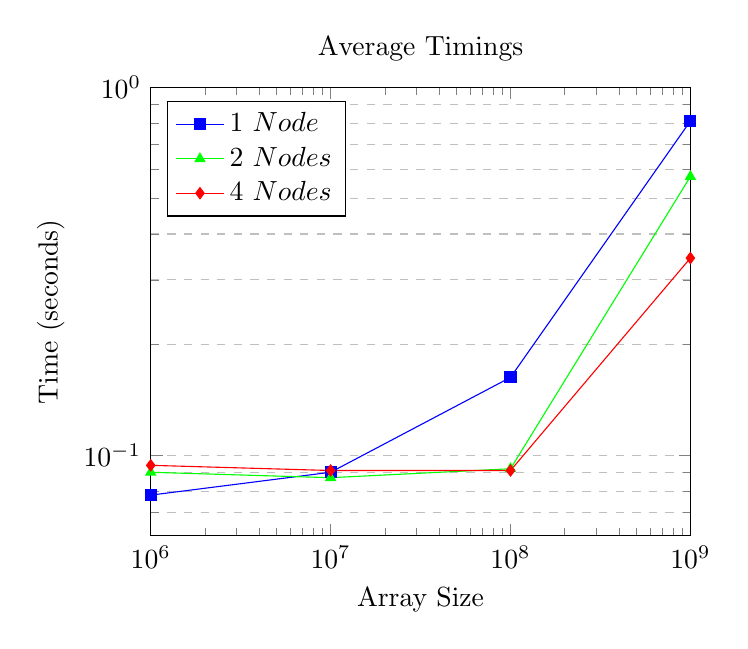
\begin{tikzpicture}
\begin{axis}[
    title={Average Timings}, xlabel={Array Size}, ylabel={Time (seconds)}, xmin=1000000, xmax=1000000000, ymin=0, ymax=1, xmode=log, ymode=log,legend pos=north west,ymajorgrids=true,yminorgrids=true,grid style=dashed,]%ytick={0, .1, .2, .3, .4, .5, .6, .7, .8, .9, 1.0},]
\addplot[color=blue, mark=square*,]
        coordinates{(1000000, 0.078)(10000000, 0.090)(100000000, 0.163)(1000000000,0.811)}; 
\addplot[color=green, mark=triangle*,]
        coordinates{(1000000, 0.090)(10000000,0.087)(100000000,0.092)(1000000000,0.573)}; 
\addplot[color=red, mark=diamond*,]
       coordinates{(1000000,0.094)(10000000,0.091)(100000000,0.091)(1000000000,0.344)}; 
\legend{$1\ Node\phantom{s}$, $2\ Nodes$, $4\ Nodes$}
\end{axis}
\end{tikzpicture}
\caption{Average Timings for Binary Search}
\label{fig:timings}
\end{figure}

For the case of $10^{6}$, using a single node was faster than the other two cases, which is most likely due to the communication costs at the beginning and end of the algorithm. However, as the size of the array increased, for $N = 10^{8}$ there was a 2-times speedup for both 2 and 4 nodes when compared to a single node. At $N=10^{9}$, there was roughly a 2-times increase in speed for using 2 nodes and roughly a 3.5-times increase in speed for using 4 nodes. This shows the scalability of the algorithm only achieved any usefulness for $N > 10^{7}$, which is likely due to the $\BigO{\log(N)}$ complexity of the Binary Search algorithm, so there wouldn't be significant gains that would be able to be seen until the constraint $\BigO{\log(N)} > \BigO{\log\left(\frac{N}{p}\right)+\log(p)}$ was met, where the $\log(p)$ term comes about due to the communication costs.

From these results, we can calculate the {\em Strong Scaling} and {\em Weak Scaling}, which can be seen in Table~\ref{table:scaling}

\begin{table}[H]
\centering
\caption{Strong and Weak Scalability}
\begin{tabular}{c c c c c}
\hline\hline
$Nodes$ & $N = 1,000,000$ & $N = 10,000,000$ & $N = 100,000,000$ & $N = 1,000,000,000$\\
\hline
\multicolumn{5}{c}{Strong Scaling}\\
\hline
2 & 43.33\% & \phantom{1}51.72\% & \phantom{1}88.59\% & \phantom{1}70.77\%\\
4 & 20.74\% & \phantom{1}24.73\% & \phantom{1}44.78\% & \phantom{1}58.94\%\\
\hline
\multicolumn{5}{c}{Weak Scaling}\\
\hline
2 & 86.67\% & 103.45\% & 177.17\% & 141.54\%\\
4 & 82.98\% & \phantom{1}98.90\% & 179.12\% & 235.76\%\\
\hline\hline
\end{tabular}
\label{table:scaling}
\end{table}
\end{solution}

\end{questions}
\begin{thebibliography}{99}
\bibitem{qselect}James Aspnes, Yale, \url{http://www.cs.yale.edu/homes/aspnes/pinewiki/QuickSelect.html}
\end{thebibliography}

\end{document}

%%% Local Variables:
%%% mode: latex
%%% TeX-master: t
%%% End:
